% Modelo desenvolvido por Amanda Luiza

% Este documento tem como intuito servir de modelo para a produção
% de documentos acadêmicos. Nele são explorados brevemente exemplos
% para inclusão de recursos como figuras, tabelas, blocos e outros
%mais.

% Adaptado de um modelo anterior construído pela autora para defesa
%de monografia.



% --- Configurações ---
% Apresentações em widescreen.
\documentclass[aspectratio=169]{beamer}	

% Tema.
\usetheme{Pittsburgh}
% Cores.
\usecolortheme{orchid}
% Fonte modo matemático.
\usefonttheme[onlymath]{serif} 
% Para mais temas e cores, consulte http://www.hartwork.org/beamer-theme-matrix/

% Customizações de Cores: fg significa cor do texto e bg, cor do fundo.
% Texto normal.
%\setbeamercolor{normal text}{fg=black}
% Texto de alerta.
%\setbeamercolor{alerted text}{fg=red}
% Autor.
%\setbeamercolor{author}{fg=blue}
% Instituto.
%\setbeamercolor{institute}{fg=blue}
% Data.
%\setbeamercolor{date}{fg=green}
% Título do slide.
%\setbeamercolor{frametitle}{fg=red}
% Subtítulo do slide.
%\setbeamercolor{framesubtitle}{fg=brown}
% Bloco padrão:
% Título do bloco.
%\setbeamercolor{block title}{bg=cyan, fg=white}
% Corpo do bloco.
%\setbeamercolor{block body}{bg=cyan!10}
% Bloco de alerta:
% Título do bloco.
%\setbeamercolor{block title alerted}{fg=white, bg=orange}
% Corpo do bloco.
%\setbeamercolor{block body alerted}{bg=orange!25}
% Bloco de exemplo:
% Título do bloco.
%\setbeamercolor{block title example}{fg=white, bg=teal}
% Corpo do bloco.
%\setbeamercolor{block body example}{bg=teal!25}


% Desativando os botões de navegação.
\beamertemplatenavigationsymbolsempty 

% Tela cheia.
\hypersetup{pdfpagemode=FullScreen}

%Numeração de títulos
\setbeamertemplate{caption}[numbered]

% Notas de rodapé.
\let\oldfootnote\footnote
\renewcommand\footnote[1][]{\oldfootnote[frame,#1]}

% Iniciar numeração de slides.
\addtocounter{framenumber}{-1}

% Fundo.
\usebackgroundtemplate{
  \centering
  
\includegraphics[width=\paperwidth]{FundoUFPR.png}}



% --- Pacotes ---
% Citações padrão ABNT.
\usepackage[alf]{abntex2cite}
% Idioma do documento.
\usepackage[brazil]{babel}
% Controle das cores.
\usepackage{color}
% Seleção de códigos de fonte.
\usepackage[T1]{fontenc}
% Inclusão de gráficos.
\usepackage{graphicx}
% Codificação do documento (conversão automática dos acentos).
\usepackage[utf8]{inputenc}	
% Fontes virtuais.
\usepackage{txfonts}	
% Ajuste de tabelas ao tamanho maximo do texto.
\usepackage{adjustbox}
% Alinhamento das legendas.
\usepackage[justification=centering]{caption}
% Ajuste nas legendas.
%\captionsetup{labelformat=empty}
% Justificar texto.
\usepackage{ragged2e}
% Citação
\usepackage[style=british]{csquotes}



% --- Informações do documento ---
\title[Título]{{\textbf{Um modelo \LaTeX\ para criação de Beamer}}}
\subtitle{\vspace{2pt}Apresentação de slides no para trabalhos acadêmicos da UFPR}
\author[Amanda Luiza]{}
\institute[UFPR]{}
\date{\vspace{-30pt}\today}



% --- Início do documento ---
\begin{document}
{%
	\begin{frame}[plain]
		
		\begin{center}
		\begin{minipage}{0.16\linewidth}
			\vspace{4pt}
			\flushleft
			
\includegraphics[width=2.3cm]{ufprlogo}
		\end{minipage}
		\begin{minipage}{0.45\linewidth}
			\vspace{5pt}
			{\footnotesize{\flushleft MINISTÉRIO DA EDUCAÇÃO\\ 
					UNIVERSIDADE FEDERAL DO PARANÁ\\
					SETOR DE CIÊNCIAS SOCIAIS APLICADAS\\ 
					CURSO DE CIÊNCIAS ECONÔMICAS\\}}
		\end{minipage}
		\end{center}
				
		\begin{center}      
			\vspace{-0.2cm}%
		\end{center}
		
		\titlepage
		
		\begin{center}
        \begin{minipage}[t]{0.6\textwidth}
			\vspace{-2.5cm}
			\centering
			{\textbf{\textit{Autor}:} Amanda Luiza\\
			\textbf{\textit{Orientador}:} Nome do(a) Orientador(a)}
		\end{minipage}
        \end{center}

\end{frame}
}



% --- Sumário ---
\begin{frame}{Sumário}
	\hfill
	\parbox[t]{.90\textwidth}{
		\begin{minipage}[c][0.75\textheight]{\textwidth}
			\tableofcontents
		\end{minipage}
	}
\end{frame}



% --- Sumário entre as seções ---
%\AtBeginSection[]{
%	\begin{frame}{Sumário}
%		\hfill
%		\parbox[t]{.90\textwidth}{
%			\begin{minipage}[c][0.75\textheight]{\textwidth}
%				\tableofcontents[currentsection]
%		\end{minipage}}
%	\end{frame}
%}



% --- Introdução ---
\section{Introdução}
\begin{frame}{Introdução}
	
	\justifying Este modelo foi elaborado com o intuito de difundir e facilitar a utilização de documentos LateX para criação de apresentações de slides (Beamer) para trabalhos acadêmicos da UFPR (Universidade Federal do Paraná).

\end{frame}



% --- Alguns exemplos ---
\section{Alguns exemplos}
\subsection{Itemização e enumeração}
\begin{frame}{Alguns exemplos}{Itemização e enumeração}
	
	\begin{itemize}
		\item \justifying Exemplo de itemização:
		\begin{itemize}
		    \item \justifying Exemplo de subitemização;
		    \item \justifying Outro subitem.
		\end{itemize}
	\end{itemize} \vspace{10px}
	
	\begin{enumerate}
	    \item \justifying Exemplo de enumeração;
	    \item \justifying Outro exemplo de enumeração.
	\end{enumerate}
	
\end{frame}



% --- Alguns exemplos ---
\subsection{Figuras}
\begin{frame}{Alguns exemplos}{Figuras}
	
	 \begin{figure}[h!]
		\centering
		\caption{Exemplo de figura}
		\label{f:figura-1}
		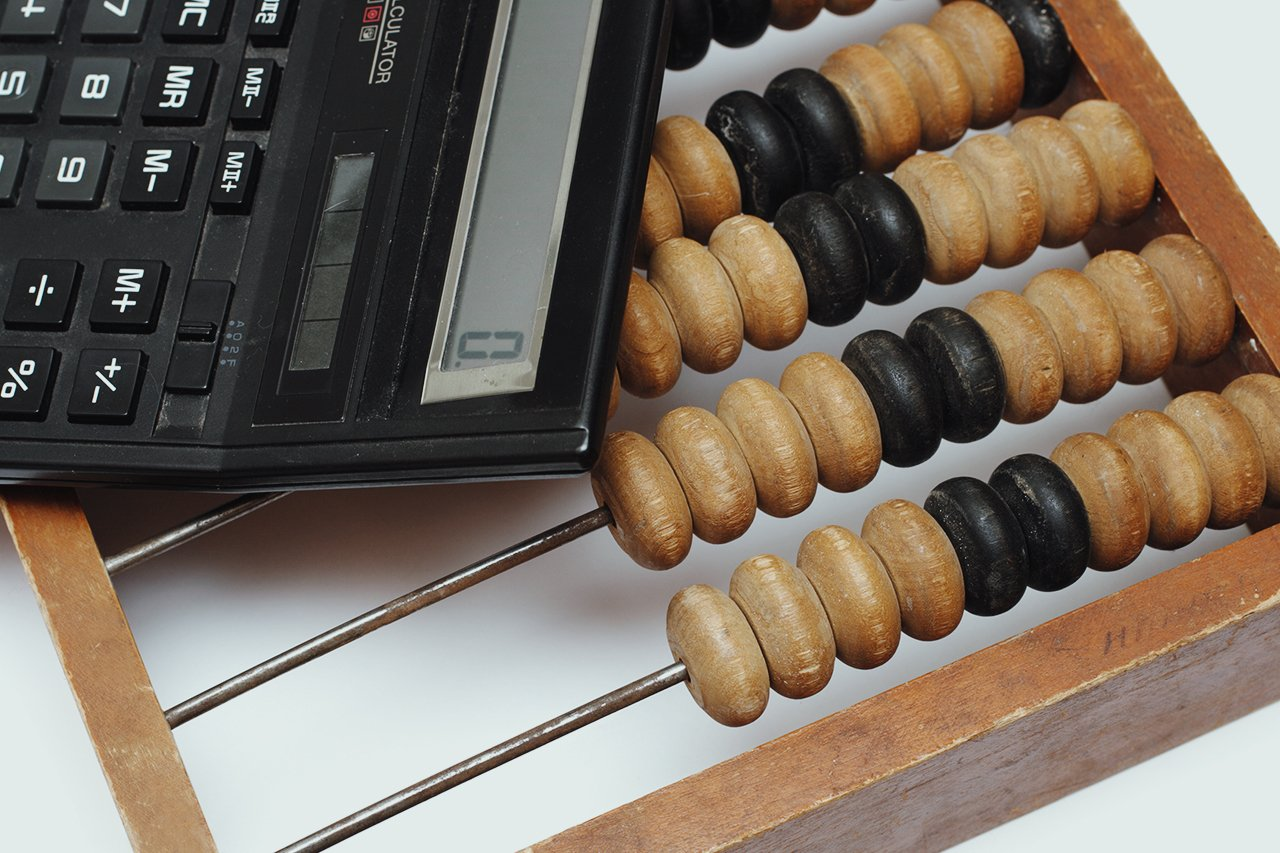
\includegraphics[scale=0.15]{figura-1.jpg}
		\parbox{10.5cm}{\caption*{\tiny{FONTE: Adicionar fonte.}}}
	\end{figure}
	
\end{frame}



% --- Alguns exemplos ---
\begin{frame}{Alguns exemplos}{Figuras}
	
	\begin{figure}[h!]
		\centering
		\begin{minipage}{0.5\textwidth}
			\centering
			\caption{Outro exemplo de figura}
			\label{f:figura-2}
			
\includegraphics[scale=0.5]{figura-2.jpg}
			\caption*{\tiny{FONTE: Adicionar fonte.}}
		\end{minipage}
		\hspace{15pt}
		\begin{minipage}{0.40\textwidth}
			\centering
			\justifying Exemplo de texto ao lado da figura, também é possível referenciar a Figura \ref{f:figura-2}.
		\end{minipage}
	\end{figure}
	
\end{frame}



% --- Alguns exemplos ---
\subsection{Tabela}
\begin{frame}[shrink=0]{Alguns exemplos}{Tabela}
	
	\vspace{-0.3cm}
    \begin{table}[h!]
    \centering 
	\caption{Exemplo de tabela}
	\label{t:tabela} 
	\begin{tabular}{@{\extracolsep{5pt}}lccc} 
		\\[-2.8ex]\hline 
		\hline \\[-1.8ex] 
		& \multicolumn{3}{c}{Notas} \\ 
		\cline{2-4}
		\\\multicolumn{1}{c}{Nome} & \multicolumn{1}{c}{Prova 1} & \multicolumn{1}{c}{Prova 2} & \multicolumn{1}{c}{Média} \\ 
		\hline \\[-1.8ex] 
		André & 9{,}0 & 8{,}0 & 8{,}5 \\ 
		& & & \\ 
		Diana & 10{,}0 & 8{,}4 & 9{,}2 \\ 
		& & & \\ 
		Lucas & 7{,}8 & 6{,}0 & 6{,}9 \\ 
		& & & \\ 
		Mariana & 9{,}5 & 6{,}5 & 8{,}0 \\ 
		& & & \\ 
		
		\hline 
		\hline \\[-1.8ex] 
		
	\end{tabular} 
	\caption*{\tiny{FONTE: Adicionar fonte.}}
\end{table}
	
\end{frame}



% --- Alguns exemplos ---
\subsection{Blocos}
\begin{frame}{Alguns exemplos}{Blocos}

    \begin{block}{Bloco padrão}
        Este é um bloco padrão.
    \end{block}
    
    \begin{alertblock}{Bloco de alerta}
        Este é um bloco de alerta.
    \end{alertblock}
    
    \begin{exampleblock}{Bloco de exemplo}
        Este é um bloco de exemplo.
    \end{exampleblock}

\end{frame}



% --- Alguns exemplos ---
\subsection{Expressões matemáticas, citações e notas de rodapé}
\begin{frame}{Alguns exemplos}{Expressões matemáticas, citações e notas de rodapé}


Exemplo de equação:
    \begin{equation}
    \centering 
	\label{t:tabela} 
        E = m \times c^2
    \end{equation}\vspace{10px}
    
Exemplo de citação:\vspace{10px}

	\begin{quote}
		Tudo o que temos de decidir é o que fazer com o tempo que nos é dado.
	\end{quote}
	
	\begin{flushright}
		\textsc{\citeonline{Tolkien}}
	\end{flushright}\vspace{10px}
	
Exemplo de nota de rodapé\footnote{Nota de rodapé.}.

\end{frame}



% --- Introdução ---
\section{Conclusão}
\begin{frame}{Conclusão}

    \justifying Através deste modelo de Beamer e dos breves exemplos do que pode ser realizado dentro deste tipo de documento, espera-se que este material possa auxiliar na elaboração de trabalhos acadêmicos de forma mais prática e estruturada.
    
%Exemplos de referências importantes que por ventura não tenham sido citadas ao longo do documento, mas devem aparecer na bibliografia:
\nocite{latex}
\nocite{Mori}
	
\end{frame}

% ----------------- NOVO SLIDE --------------------------------
\section{Referências}

% --- O comando \allowframebreaks ---
% Se o conteúdo não se encaixa em um quadro, a opção allowframebreaks instrui 
% beamer para quebrá-lo automaticamente entre dois ou mais quadros,
% mantendo o frametitle do primeiro quadro (dado como argumento) e acrescentando 
% um número romano ou algo parecido na continuação.

\begin{frame}[allowframebreaks]{Referências}
\bibliography{referencias}
\end{frame}

% ----------------- FIM DO DOCUMENTO -----------------------------------------
\end{document}